\chapter{Технологическая часть}

В данном разделе представлены архитектура приложения, средства разработки программного обеспечения, детали реализации и способы взаимодействия с программным продуктом.

\section{Архитектура приложения}

Предполагается, что разрабатываемый сервис состоит из двух приложений: анализатор (OLAP Cube) и веб-интерфейс взаимодействия с данными, полученными из первого микросервиса. Доступ к агрегированным данным будет получен с помощью GET запросов.

Общая схема архитектура сервиса представлена на рисунке \ref{fig:arch}.

\begin{figure}[!h]
	\center{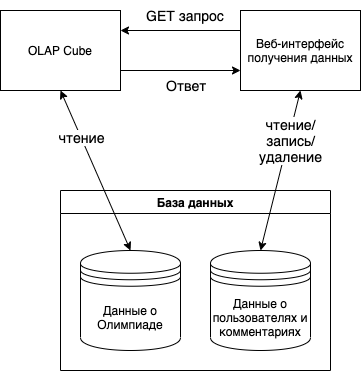
\includegraphics[scale=0.8]{img/arch.png}}
	\caption{Схема архитектуры приложения}
	\label{fig:arch}
\end{figure}

\section{Средства реализации}

Для разработки приложений был выбран язык программирования Python \cite{python}. Данный выбор
обусловлен простотой языка, его интерпретируемостью, а также тесной интеграцией с СУБД PostgreSQL \cite{python}, которая будет использоваться для хранения данных.

Для развёртыания OLAP куба был выбрана фремворк cubes \cite{cube-lib}, позволяющая развернуть куб на отдельном сервере и общаться с базой данных на основе СУБД PostgreSQL 
\cite{python} без дополнительных коннекторов или библиотек.

Для получения данных посредством GET запросов была выбрана библиотека request \cite{requests-lib}.

\section{Детали реализации}

В приложении на листингах \ref{lst:olap} -- \ref{lst:sql} приведён код взаимодействия приложений с базой данных, OLAP кубом, а также инициализации базы данных.


\section{Взаимодействие с приложением}

На рисунках \ref{fig:app1} -- \ref{fig:app3} представлены примеры работы приложения.

\begin{figure}[!h]
	\center{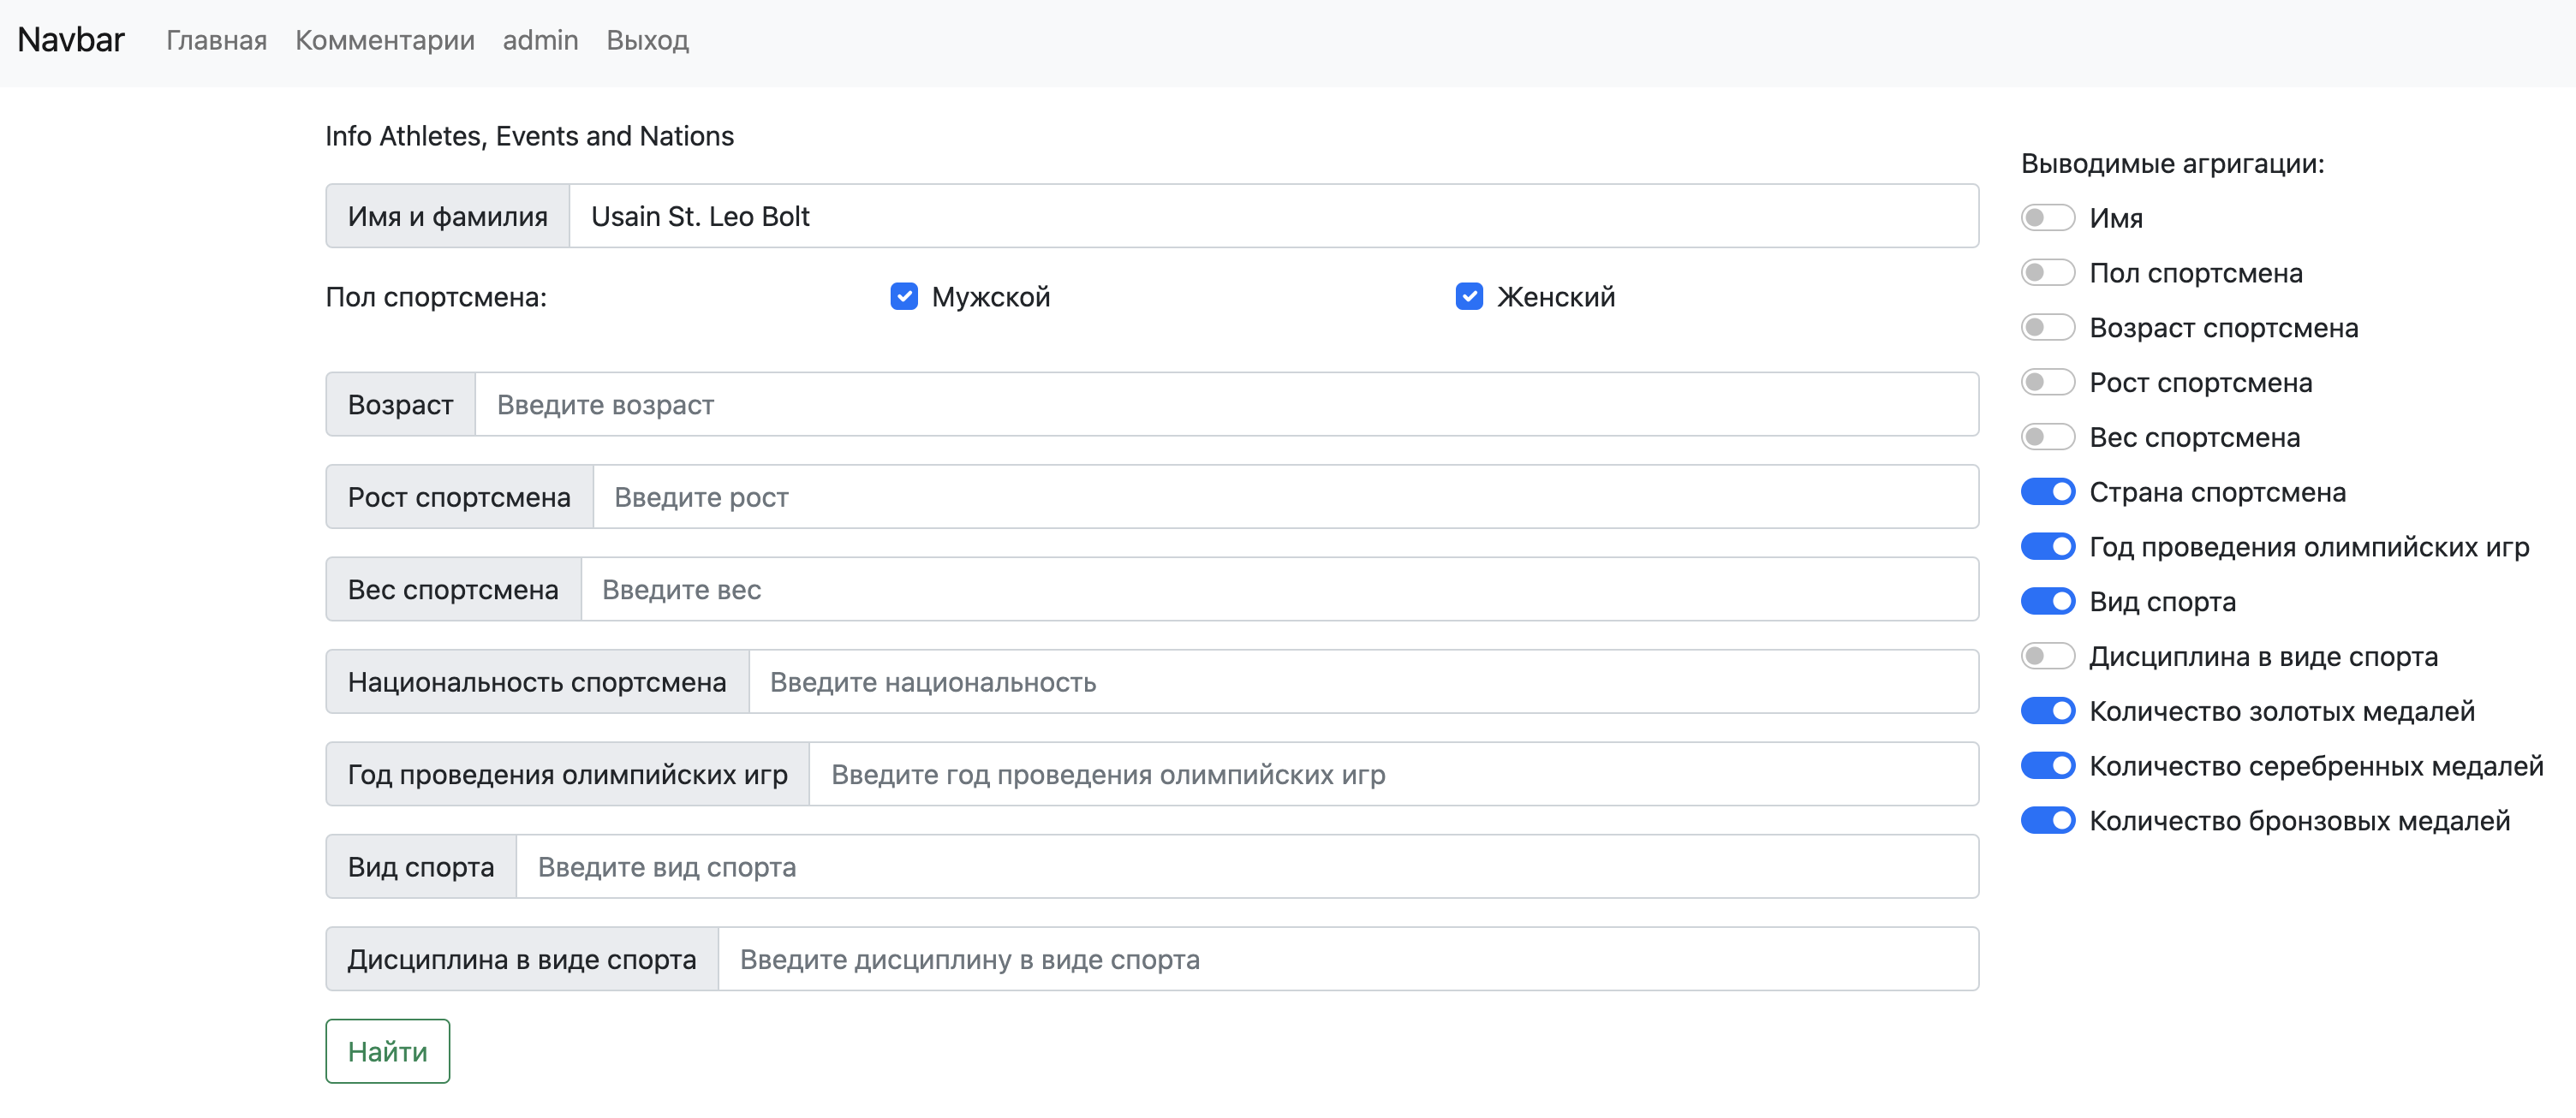
\includegraphics[scale=0.3]{img/menu.png}}
	\caption{Пример взаимодействия с интерфейсом}
	\label{fig:app1}
\end{figure}

\begin{figure}[!h]
	\center{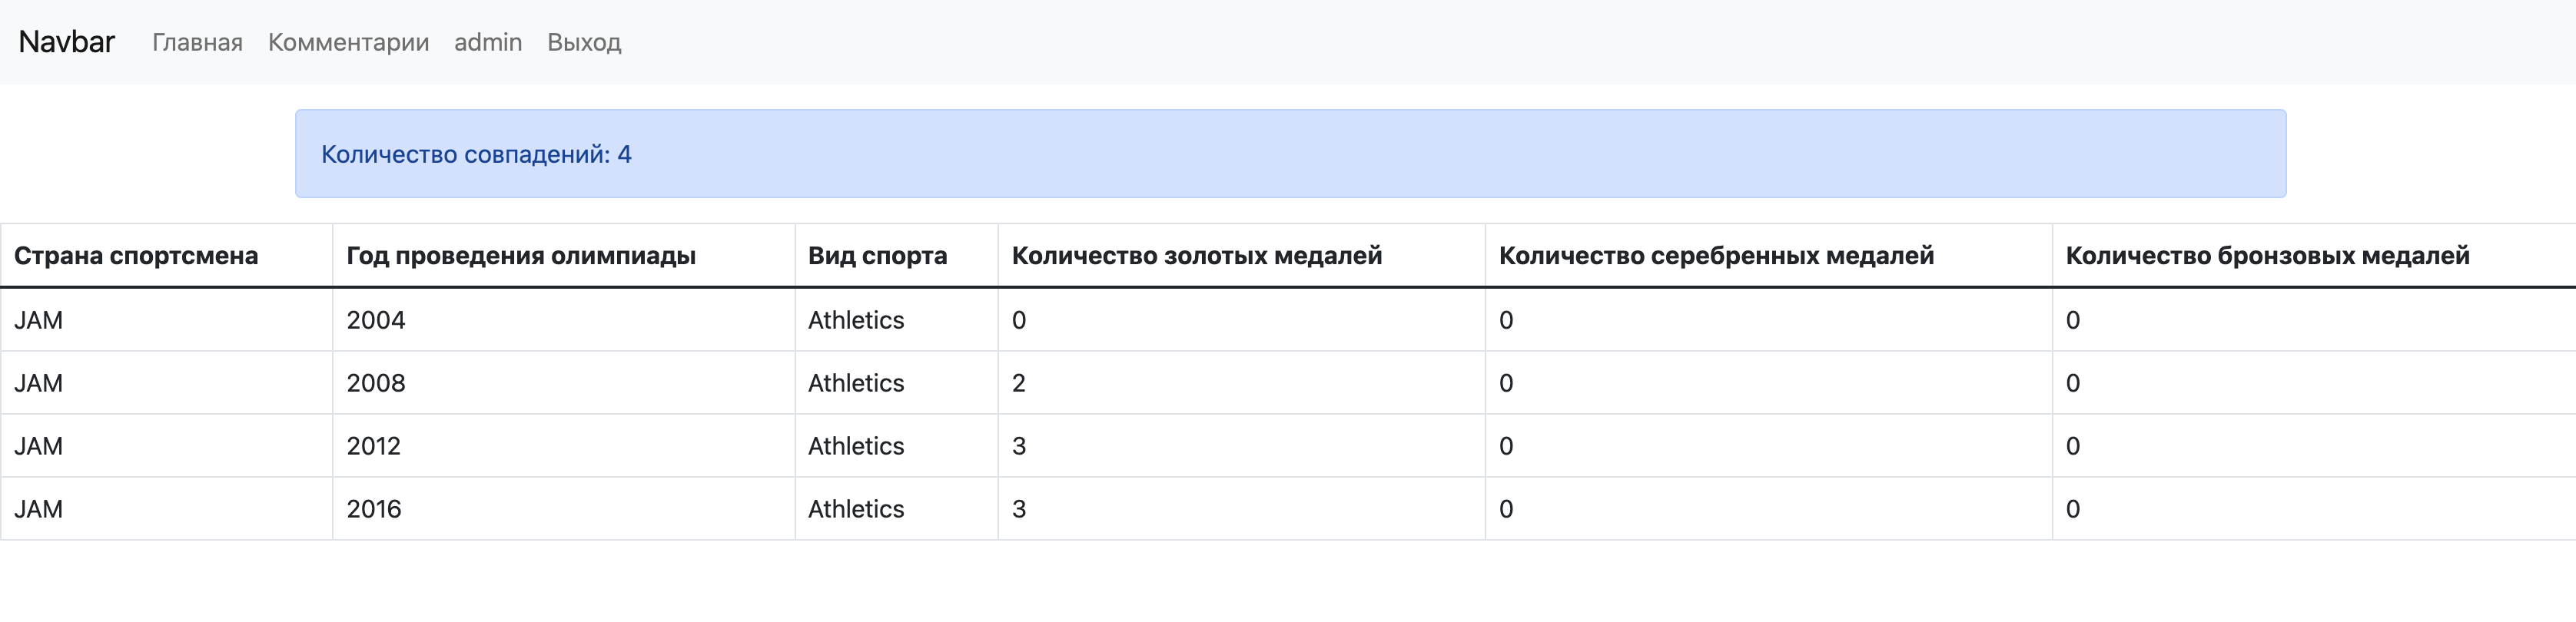
\includegraphics[scale=0.3]{img/tab_res.png}}
	\caption{Пример выдачи}
	\label{fig:app2}
\end{figure}

\begin{figure}[!h]
	\center{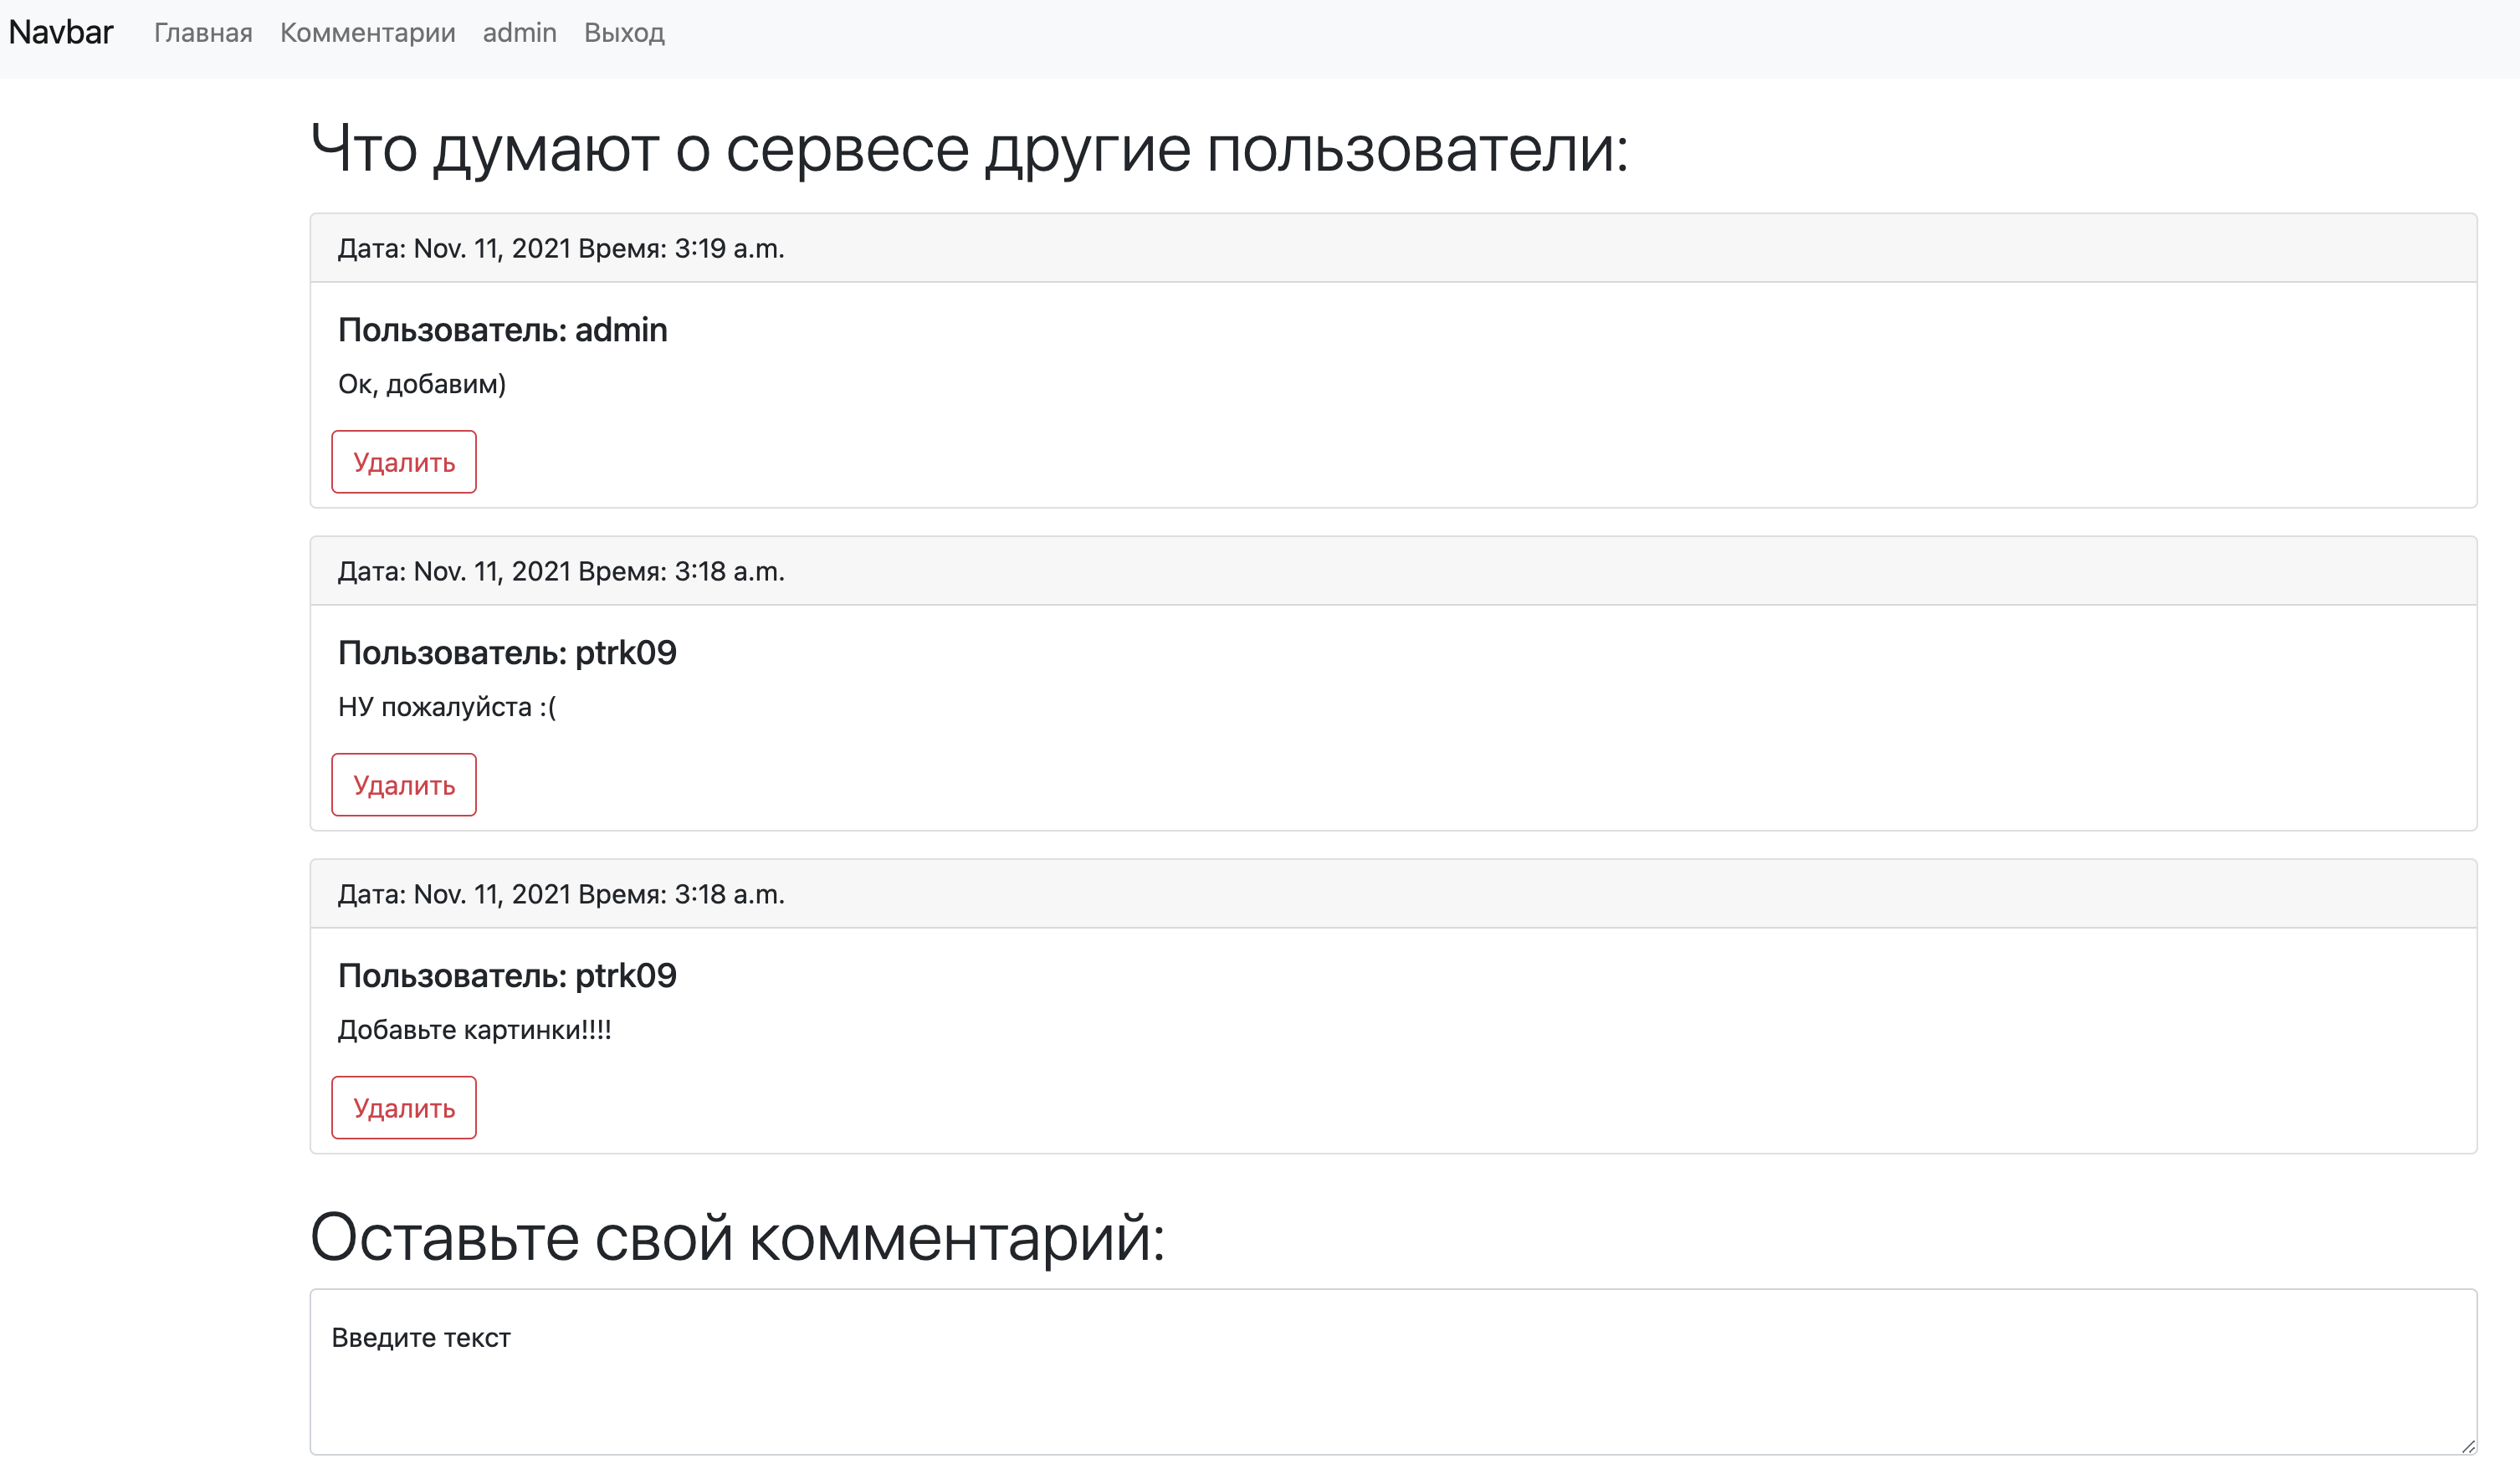
\includegraphics[scale=0.3]{img/comments.png}}
	\caption{Пример работы с комментариями}
	\label{fig:app3}
\end{figure}

\newpage

\section*{Вывод}

В данном разделе была представлена архитектура и рассмотрены средства реализации веб-сервиса, листинги ключевых компонентов системы и пример работы приложения.